\chapter{Two--Component Relativistic Electronic Structure Theory}

\section{Noncollinear Kohn--Sham Density Functional Theory}

\subsection{Discussion}
\subsubsection{Validation}
Molecular systems characterized by geometrically frustrated conformations have been used to gauge the reliability of the presented implementation, since generalized-KS  and X2C-KS, unlike U-KS, methods are capable to support the broken $\op{S}_z$ symmetry that minimizes Pauli repulsion.\cite{Gross07_196405,Frisch07_125119,Frisch12_2193,Scuseria13_035117,Yamaguchi01_670,Blochl03_15772,Truhlar11_2629,Truhlar13_5349,Li15_154109}
Thus, we examined a series
of neutral hydrogen rings, ranging from 3 to 8 hydrogen atoms, that have already been proved to show broken symmetry solutions within generalized Hartree-Fock theory.\cite{Li15_154109}
The used conformations have 1 \AA~ spaced hydrogen atoms and only the  odd-membered rings will be geometrically frustrated.
All  hydrogen rings electronic structure were obtained by solving the presented X2C-KS
equation  in open-source \texttt{ChronusQ}\cite{chronusq_beta2} electronic structure software using the hybrid Becke, 3-parameter, Lee-Yang-Parr (B3LYP) density functional 
\cite{Becke93_5648,Parr88_785,Preuss89_200} with a 6-311+g** basis, since it is required to include the polarization of hydrogenic s-functions.\cite{Li15_154109}
Qualitatively,  X2C-KS solutions are given in \cref{fig:rings}, where both the spin and the charge densities are reported, respectively. The spin density in the non-collinear
approach is a mapping of the 2-norm of the spin magnetization vector onto the total density \cite{Wullen02_779}, ensuring the spin density to be positive and always real, and the charge density is a mapping of the electrostatic potential to the total density.
For even numbered rings, the anti-ferromagnetic
spin distribution can be observed, aside from the six rings (where the closed shell solution is the most stable one according to the $2n + 1$ rule for M\"obius-like periodicity).
For odd membered rings, the M\"obius-like periodicity of magnetization ordering
in X2C-KS results can be inspected by the totally symmetric distribution of the spin density throughout the structure in \cref{fig:rings}. This symmetric distribution can not be supported by collinear solutions\cite{Li15_154109} which are constrained to be eigenfunctions of $\op{S}_z$. Thus, X2C-B3LYP  is able to reproduce the expected symmetry of non-collinear results for odd membered rings \cite{Li15_154109}, ensuring the reliability of the  current implementation.

\begin{figure}
\begin{center}
\resizebox{6.5in}{!}{%
  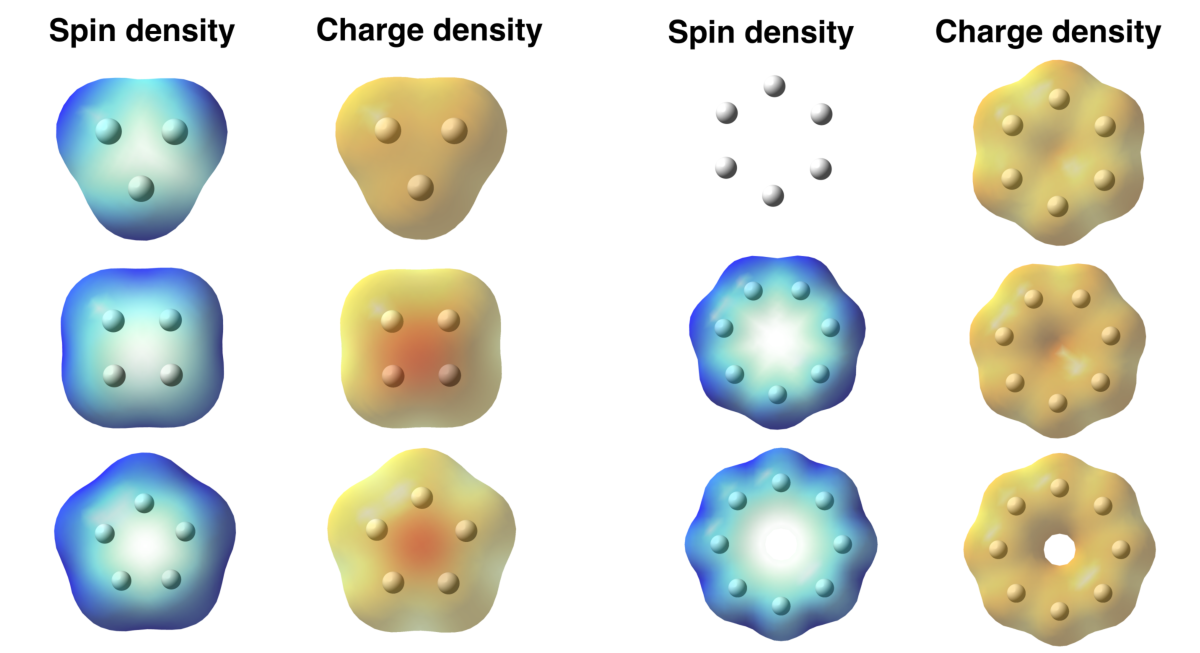
\includegraphics{rings.pdf}
}
\end{center}
\caption{X2C-B3LYP  6-311+g** spin and charge densities for hydrogen rings sizes 3-8. The spin density is represented as the 2-norm of the magnetization vector at each point in space (left, in blue largest magnitude), and the charge density as the electrostatic potential mapped to the total density (right, in red largest electronic population).}
\label{fig:rings}       
\end{figure}

\subsubsection{Performances}
\begin{figure}
\begin{center}
\resizebox{6.5in}{!}{%
  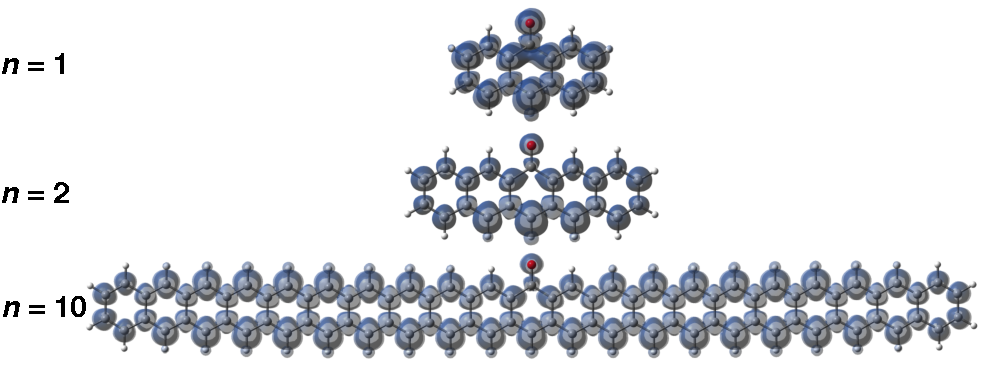
\includegraphics{radicals.pdf}
}
\end{center}
\caption{X2C-B3LYP 6-311+G(2d,p) spin densities for phenoxy radicals with increasing number of symmetrical fused benzene rings ($n$=1-10, where $n$ represents the number of fused benzene rings on each side). The spin density (here the 0.001 iso-surface) is obtained as the 2-norm of the magnetization vector at each point in space.}
\label{fig:radicals}       
\end{figure}
After we have checked the reliability and presented the schematics of the integration scheme, 
we focus on the performances of the method.
All the following tests presented are performed without exploiting symmetry using B3LYP/6-311+G(2d,p) theory level
and atomic centered grids resulting as the product of a radial and angular
quadrature, using 100 Euler-Maclaurin~\cite{Laming93_997}, and 302 Lebedev (l = 29)~\cite{Lebedev77_99} grid points, respectively (100$\times$302 grid).
All calculations were performed using Intel Haswell compute nodes (14$\times$2 Intel\textregistered Xeon E5--2680 v4 CPUs @ 2.40 GHz, 32k L1 cache, 256k L2 cache, 35840k L3 cache).
All times refer to the combined wall time for 
the numerical evaluation of $E_{XC}$ and the matrix elements  $V^{GGA,I}_{\mu\nu}$, (\cref{eq:EXCGGA_num} and \cref{eq:VXCGGA_num}) for
each  self consistent field (SCF) step (as average over 5 steps).
The scaling of the numerical integration
with respect to increasing system sizes is investigated first by measuring wall timings on a series of phenoxy radicals with increasing number of symmetrical fused benzene rings ($n$=1-10). 
These systems have been chosen, since they present a delocalized spin-density over the entire molecule (see \cref{fig:radicals}) for all values of $n$. This is very important, since the screening based on the different components of the density can be very large in regions showing zero magnetization density.
Wall times are shown in \cref{fig:timing} as function of the total number of atoms in the systems for both the U-KS and X2C-KS implementations.
The scaling factors are similar for both U-KS and X2C-KS integration (see the parallel fitted lines in the figure), showing how the  X2C-KS integration does not show any consistent computational overhead in the   $V^{GGA,I}_{\mu\nu}$ integration with
respect to the common U-KS integration. 
Finally, by employing the largest phenoxy radical of the series ($n$=10), the same wall times are recorded as function of increasing MPI processes across different computational nodes (for 1, 2, 4, 8, 12 nodes, for a total 
of 28, 56, 112, 224, 336 CPUs) and reported in \cref{fig:nodes}. 
The implemented algorithm presents linear ($-1.01$) with increasing number of CPUs, as can be expected since the integration over different atomic centers can be easily independently performed across different computing nodes.
\begin{figure}
\begin{center}
\resizebox{3.25in}{!}{%
  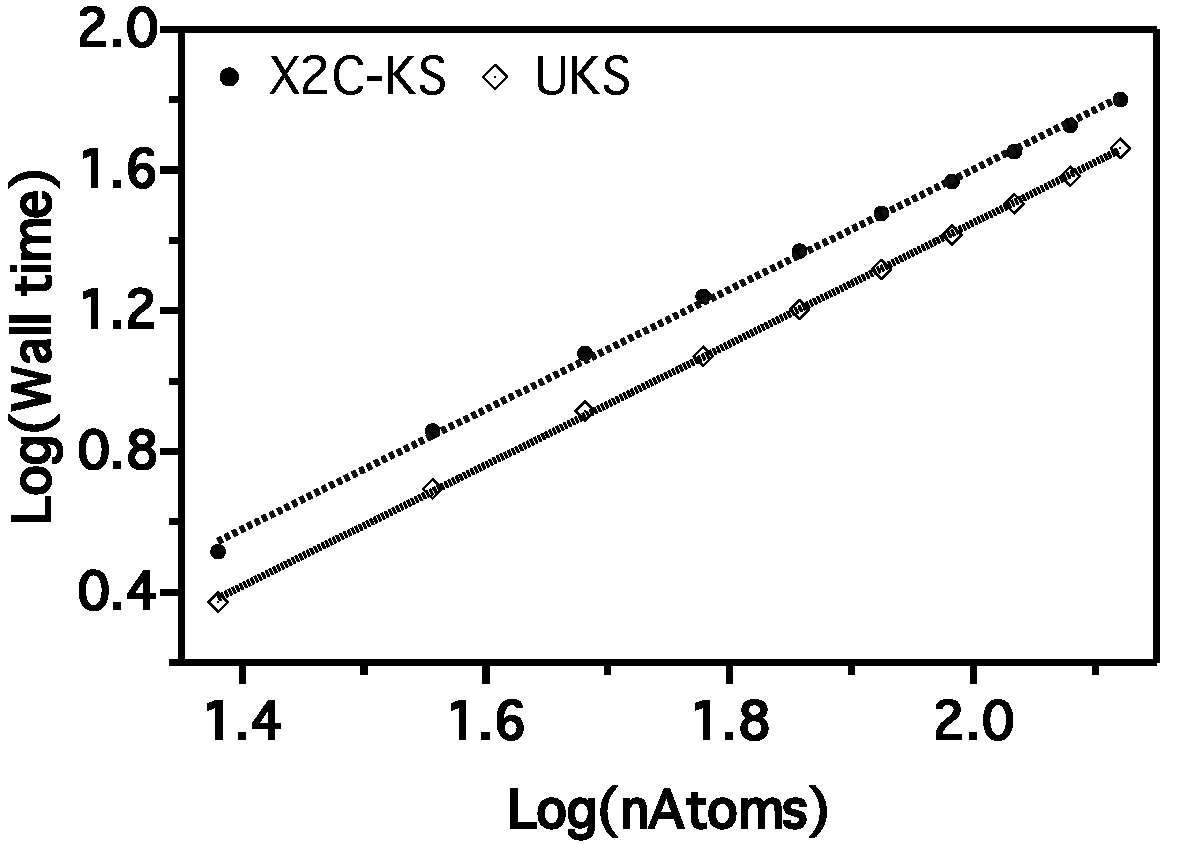
\includegraphics{timings_natoms.pdf}
}
\end{center}
\caption{Wall timings in seconds as a function of the total number of atoms in the systems for the evaluation of the $E_{XC}$ and the matrix elements $X_{\mu \nu}$ in one SCF step (as average over 5 steps, 6-311+G(2d,p), 100$\times$302 grid.
  Both the U-KS, empty diamonds, and X2C-KS, filled circles, are reported for comparison. A linear fit in this log-log scale is performed to show the similar scaling for the two different integration. 
}
\label{fig:timing}     
\end{figure}

\begin{figure}
\begin{center}
\resizebox{3.25in}{!}{%
  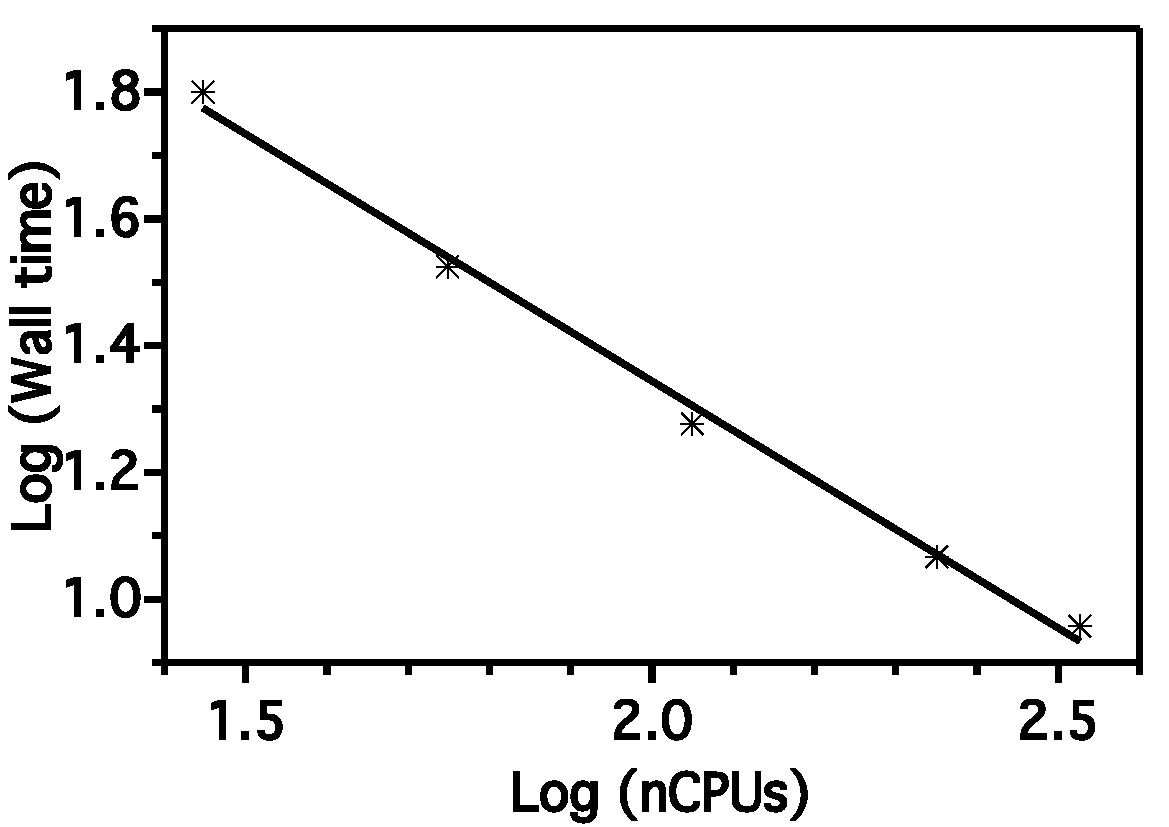
\includegraphics{cpus.pdf}
}
\end{center}
\caption{
Wall timings in seconds as function of increasing computational CPUs of the $E_{XC}$ and the matrix 
elements $X_{\mu \nu}$ for each SCF step (as average over 5 steps, 6-311+G(2d,p), 100$\times$302 grid, 
2619 basis functions). A linear fit, -1.01 slope, is also represented as full line.
}
\label{fig:nodes}       
\end{figure}

\subsection{Conclusions}
In this work, we presented an integration and assembly strategy, 
using a two-component spinor density, for efficient evaluation
of the exchange correlation term using localized basis
functions. 
The presented formulation is suitable to exploit parallelism 
along with optimal cache utilization and micro-architecture specific floating point operations.
This leads to the evaluation of exchange correlation
contributions with matrices of optimal sizes. 
We also show that the proper choice of auxiliary variables 
correctly give rise to nonzero local torque of the xc magnetic field on the magnetization
while maintaining net zero global torque, as is expected from
the exact functional. 
Several tests were used to validate 
the reliability and the performance of the proposed strategy.
This approach can help to extend 
the applicability of relativistic two-component DFT 
to systems of large size ($>$ 100 atoms). 







\section{The Relativistic Particle--Particle Random Phase Approximation}



\subsection{Results and Discussion}
\label{sec:Results}

\co{This section needs heavy revision to cite internal sections as opposed to papers}
All calculations were performed with a locally modified version of the Gaussian quantum chemistry suite of programs,\cite{GDVI06}
and employed the taug-cc-pVTZ-DK basis set\cite{Dixon01_48} with the diffuse \emph{f}-functions removed.
Relativistic effects were accounted for by means of the variational X2C method \co{Specific HF}.\cite{Reiher13_184105,Saue11_3077,Liu09_219,Liu10_532,Liu09_1945}
In order to partially account for two-electron spin-orbit interaction in the Hamiltonian, we employed a scheme based on the scaling of the nuclear charge according to the angular momenta.\cite{Boettger00_7809}
The atomic nuclei, rather than being treated as point charges, were described using $s$-type Gaussian charge distribution.\cite{Dyall97_207,Saue98_920}
The stability of the two-component ground state wave function was also tested before X2C-pp-TDA calculations were performed.\cite{Li15_154109}

\subsubsection{Single Excitations}
\label{subsec:SingleEx}
In order to highlight the capability of the pp-TDA method to describe excited
states within a relativistic framework, in this section we examine the fine
structure splittings of some atomic systems.  The presence of spin-orbit
couplings 
%causes the total spin, $\vec{S}$, and orbital, $\vec{L}$, angular
%momentum operators to no longer commute with the Hamiltonian, therefore they no
%longer generate good quantum numbers for the system.  Instead, the total
%angular momentum $\vec{J}=\vec{L}+\vec{S}$ is the fundamental quantity that
%should be considered when classifying the electronic states of the system.  A
%direct consequence of spin-orbit couplings on the spectra of atoms is the
%lifting of some of 
lifts some of the energetic degeneracies that would be expected in the ground or
excited electronic states.  We therefore calculate the \ch{spectrum}{excitation energies} of selected
atomic systems and compare the obtained fine structure splittings with
experimental reference values\cite{NIST_ASD} to asses the accuracy of the
method.  In this section we restrict ourselves to states describable by single
excitations (with respect to the $N$-electron system) which allows us to also
compare our results with the results obtained using the two-component
particle-hole Random-Phase Approximation (X2C-ph-RPA), also known as
Time-Dependent Hartree-Fock method (X2C-TDHF), as well as with results obtained
using the X2C-ph-TDA method.\cite{Li16_3711} Results for these fine-structure
splittings are collected in \cref{tb:SingleEx}.

It can be seen that, in general, the three methods perform similarly with
respect to the reference values insofar as the order of magnitude of the error
is concerned. A general trend may be observed in that the X2C-pp-TDA
consistently overestimates the splittings as the atomic charge of the
underlying nucleus increases. This effect is magnified in the low energy
transitions while it is less apparent in the higher energy transitions. This is
due to the fact that the frontier orbitals of the ($N-2$)-reference being used
become sub-optimal in the proper description of the $N$-electron system due to
a contraction in the presence of higher nuclear charge. This leads to an
unphysically small energetic separation between the frontier orbitals of the
$N$-electron system which causes increasing errors due to an unphysical
increase in mixing. This problem is less obvious in higher energy excitation
because the higher lying orbitals are not as affected. These orbitals are
properly optimized in the X2C-ph-RPA/TDA due to orbital occupancy of the
resulting wave function. The general out-performance of the X2C-ph-TDA over the
X2C-ph-RPA may be attributed to an over estimation of electron correlation in
the ground and excited states via the RPA\cite{Dreuw05_4009}. The presence of
the de-excitation amplitudes in the X2C-ph-RPA allow for an over-mixing for the
low-lying excited states with the ground state which give rise to an
overestimate of the FSS, much the same as the case for the X2C-pp-TDA.
                                                                                                                                                 
 
                                                                                                                                                                                                                                                              
 
The main advantage of the particle-particle over the particle-hole formalism is
that, in the former, both the ground and electronically excited $N$-particle
states are described on equal footing with respect to correlation, being a
linear combination of several Slater determinants.  Conversely, in the ph-TDA
or ph-RPA method, the ground state is described as a single determinant, while
excited states are described as linear combinations of single excitations (and
possibly de-excitations).  That being said, the excitation space spanned by the
X2C-pp-TDA solutions does not include all chemically relevant excitations, many
of which can be found using the more traditional ph-RPA or ph-TDA methods.
This is due to the fact that the X2C-pp-TDA is, in its traditional form,
incapable of accessing excitations that involve contributions from below the
Fermi level.  Some work has been done in attempts to resolve this
problem\cite{Yang13_224105}, but these alterations to the pp-TDA method have
not been explored in this work.

\begin{table}[htbp]
  \caption{Calculated and reference\cite{NIST_ASD} excited-state fine structure splittings (in meV) of some atomic systems. The presence of a superscript ``$\circ$" in the term symbol denotes an odd state with respect to space inversion.}
 \label{tb:SingleEx}
 \centering
 \begin{tabular}{llrrr}
  \hline
  Method     & Level                                              &  Mg   & Al$^+$ & Si$^{2+}$ \\ \hline
  X2C-ph-RPA & \multirow{3}{*}{$^3$P$^\circ_{1}-^3$P$^\circ_{0}$} &  4.89 & 10.49  & 19.85 \\
  X2C-ph-TDA &                                                    &  2.41 &  7.94  & 16.62 \\
  X2C-pp-TDA &                                                    &  2.77 &  9.13  & 18.97 \\
  Ref        &                                                    &  2.49 &  7.55  & 15.94 \\
  \hline
  X2C-ph-RPA & \multirow{3}{*}{$^3$P$^\circ_{2}-^3$P$^\circ_{1}$} &  9.75 & 21.02  & 39.96 \\
  X2C-ph-TDA &                                                    &  4.82 & 15.96  & 33.50 \\
  X2C-pp-TDA &                                                    &  5.55 & 18.40  & 38.40 \\
  Ref        &                                                    &  5.05 & 15.36  & 32.45 \\
  \hline
  X2C-ph-RPA & \multirow{3}{*}{$^3$P$^\circ_{1}-^3$P$^\circ_{0}$} &  0.33 &  1.82  &  4.43 \\
  X2C-ph-TDA &                                                    &  0.33 &  1.82  &  4.31 \\
  X2C-pp-TDA &                                                    &  0.42 &  2.17  &  5.08 \\
  Ref        &                                                    &  0.41 &  1.73  &  4.10 \\
  \hline
  X2C-ph-RPA & \multirow{3}{*}{$^3$P$^\circ_{2}-^3$P$^\circ_{1}$} &  0.67 &  3.67  &  9.09 \\
  X2C-ph-TDA &                                                    &  0.67 &  3.68  &  8.86 \\
  X2C-pp-TDA &                                                    &  0.84 &  4.50  & 11.04 \\
  Ref        &                                                    &  0.84 &  3.65  &  9.07 \\ 
  \hline
  \\
  \\
             &  &  MSE  &  MAE   & \\
  \hline
  X2C-ph-RPA &  &  2.32 &  2.28  & \\
  X2C-ph-TDA &  &  0.32 &  0.19  & \\
  X2C-pp-TDA &  &  1.55 &  1.55  & \\
  \hline
 \end{tabular}
\end{table}

\subsubsection{Triplet References and Double Excitations}
\label{subsec:DoubleEx}
In this section we wish to highlight other advantages of X2C-pp-TDA over conventional X2C-ph-RPA.
In the previous section we presented results for atomic systems that are characterized by being closed shell in both the $N$ and $N-2$ systems.
This is important because if the reference state has unpaired electrons then, as a consequence of the single reference nature of the Hartree-Fock wave function,
excited states will in general be spin-contaminated, affecting one's ability to extract meaningful fine structure splittings from the results, though adaptations to the general case exist.\cite{Liu10_064106,Suo11_134101,Liu11_194106,Liu12_024107,Liu13_3741}
By using X2C-pp-TDA it is however possible to treat systems with $N$ electrons with any odd spin multiplicity, provided they become closed shell upon the addition or removal of two electrons.
Molecules which possess triplet ground states as well as diradical moieties may be taken as examples.
To demonstrate this feature we compare the FSS of one set of excited states of molecular oxygen with experimental data in \cref{tb:DoubleEx}.
The difference between the calculated and measured value is just 2.5~meV, notwithstanding the approximations intrinsic in our method (e.g.~the approximate treatment of electron correlation and the two-electron spin-orbit contributions, or the finite basis set).
Of course, the same reasoning can also be applied in reverse: X2C-ph-RPA theory can be readily used to find excited-state FSS of systems with a singlet ground state, however if the addition or removal of two electrons produces an open-shell molecule, then X2C-pp-TDA will present some spin-contamination in the computed excited-states.



One advantage that X2C-pp-TDA always has over X2C-ph-RPA theory, however, is its ability to describe double excitations.
\Cref{tb:DoubleEx} compares calculated and reference excited-state FSS of doubly-excited states of some atomic moieties.
The performance of the method is similar as in the case of single excitations presented in the previous section.
Such states cannot be found among the excited states computed via X2C-ph-RPA.

\begin{table}[htbp]
 \caption{Excited-state fine structure splittings (in meV).}
 \label{tb:DoubleEx}
 \centering
 \begin{tabular}{llrr}
  \hline
  System & Level & X2C-pp-TDA & Ref \cite{NIST_ASD,Krupenie72_423} \\ \hline
  O$_2$ & $^3\Delta_3-{^3\Delta_2}$ & 20.58 & 18.09 \\ \hline
  \multirow{2}{*}{Al$^+$} & $^3$P$_1-^3$P$_0$ & 9.20 & 7.75 \\ 
  & $^3$P$_2-^3$P$_1$ & 17.93 & 15.03 \\  \hline
  \multirow{2}{*}{Si$^{2+}$} & $^3$P$_1-^3$P$_0$ & 19.46 & 16.55 \\ 
  & $^3$P$_2-^3$P$_1$ & 37.88 & 32.06 \\    \hline
 \end{tabular}
\end{table}

%-------------------------------------------------------------------------------
% CONCLUSION
%-------------------------------------------------------------------------------
\subsection{Conclusion}

In this work, a scheme for the extension of the pp-TDA method to relativistic two-component wave functions has been presented.
This scheme involves the approximate decoupling of the large and small components of the relativistic wave function by means of the X2C method, followed by an Hartree-Fock SCF calculation on the system obtained by removing two electrons, in order to obtain a set of complex spinor molecular orbitals.
The two-component reference system is then used in the X2C-pp-TDA calculation that yields the ground and excited states for the $N$-electron system.
The extension of the pp-TDA to a two-component reference comes at the cost of the employing complex spinor orbitals, and not being able to separate the problem into smaller sub-problems as is done in the case of RHF or UHF references via spin integration.
The increased computational cost highlights the ever pressing need for direct and parallel implementations of post-SCF electronic structure methods, which is exaggerated in the case of relativistic electronic structure calculations.

It has been shown that the X2C-pp-TDA method exhibits excellent results in the prediction of the fine-structure splittings of the atomic and molecular species considered here.
The results are comparable and at times better than those obtained using X2C-ph-RPA.\cite{Li16_3711}
In addition, the X2C-pp-TDA is able to capture electronic excitations traditionally inaccessible by the X2C-ph-RPA/TDA thanks to the 2-particle reference shift, such as double excitations and those that would be described as spin-contaminated in particle-number conserving methods.
While these results are promising, the general applicability of the X2C-pp-TDA method, as with the spin-collinear variant, is limited as it is traditionally unable to capture excitations that involve contributions of orbitals from below the Fermi level.
That being said, there are many systems, such as triplet and diradical systems, that the X2C-pp-TDA provides a suitable method for the accurate description of the
electronic manifold.

